% !Mode:: "TeX:UTF-8"
% !TEX program  = xelatex

\documentclass[bwprint]{gmcmthesis}
% \documentclass[bwprint,fontset=fandol]{gmcmthesis} % Overleaf 等在线平台需要用这一行。
\usepackage[framemethod=TikZ]{mdframed}

\usepackage{subfig}
\usepackage{colortbl}
\definecolor{color1}{rgb}{0.78,0.88,0.99}
\definecolor{color2}{rgb}{0.36,0.62,0.84}
% \definecolor{color3}{rgb}{0.8235,0.8706,0.9373}
\definecolor{color3}{rgb}{0.88,0.92,0.96}
\definecolor{color4}{rgb}{0.96,0.97,0.98}   % {0.9176,0.9373,0.9686}

% 算法
\usepackage[noend]{algpseudocode}
\usepackage{algorithmicx,algorithm}
\floatname{algorithm}{算法}
\renewcommand{\algorithmicrequire}{\textbf{输入:}}
\renewcommand{\algorithmicensure}{\textbf{输出:}}
% \numberwithin{equation}{section}
% \numberwithin{figure}{section}
% \numberwithin{table}{section}
\newcommand{\red}[1]{\textcolor{red}{#1}}
\newcommand{\blue}[1]{\textcolor{blue}{#1}}


\title{算力约束下提升大语言模型能力的资源配置建模}   % 标题
\baominghao{4321}   % 参赛队号
\schoolname{男男大学}   % 学校名称(跨校加角标$^1$标注对应关系)
\membera{队员A}   % 队员A(跨校加角标$^1$标注对应关系)
\memberb{队员B}   % 队员B(跨校加角标$^1$标注对应关系)
\memberc{队员C}   % 队员C(跨校加角标$^1$标注对应关系)
\begin{document}

% 生成标题
\maketitle


\begin{abstract}    % 摘要
    数学建模
    \keywords{模板\quad  \LaTeX{}\quad   数学建模}    % 关键字
\end{abstract}

\pagestyle{plain}

\tableofcontents    % 目录


\section{问题重述}  % 1
\textbf{问题一：}

附件 A 给出两类数据。

第一类为 A1--A3 的质量信号数据，每条文本包含 22 个质量指标，其中既有教育价值、流畅度、可读性等正向指标，也有广告概率、重复比例等负向指标，还有文本长度、数字比例等不宜简单假定单调优劣的指标。题目要求使用 A1 抽样集以及 A2、A3 扩展集的全部记录，建立样本级和领域级质量评分 $Q$，并检验扩展集与抽样集是否具有一致结论。当不同指标对同一文本给出显著不一致的判断时，还需定义冲突、分析来源并提出消解方法。

第二类为 A4--A15 的 RegMix 配方实验数据。每个配方由 17 个 The Pile 子领域的份额构成，份额非负且和为 1；对应结果为 13 个验证领域的交叉熵 Loss。需要利用 A4/A5 建模，在 A6--A11 的 1M、60M、1B 检验集上验证，并利用 A12--A15 讨论 10B 和 70B 外推结论的稳健性。由于质量信号领域和配方领域并不完全一致，若将 $Q$ 引入配比模型，必须说明映射、可辨识性和不确定性。


\section{模型假设}  % 2
\begin{enumerate}[label=\textbf{H\arabic*.},leftmargin=2.5em]
    \item 附件中标记为真实的数据能够代表对应数据源；半合成、子集和外推数据按其标记使用，不与真实实验混同。
    \item 二分类列表的末位为正类 logits，ModernBERT 六维输出的类别顺序与质量等级一致；若原始模型标签顺序相反，应在代码配置中同步调整。
    \item A1 可作为 22 个质量指标归一化和权重估计的参考样本，A2/A3 只用于扩展验证和相应领域最终评分。
    \item 配比表中的舍入误差可通过闭合操作修正；加入小伪计数后，零份额的对数比可以稳定计算。
    \item 二次响应面只解释观测配方邻域内的关联效应，有限差分不被解释为全局因果效应。
    \item 不同参数规模改变绝对 Loss 基准，但配方优劣排序可能迁移，因此跨规模以秩相关为主要评价标准。
\end{enumerate}


\section{定义与符号说明}   % 3
\begin{table}[H]    % table 3.1
    \centering
    \caption{主要符号}
    \label{tab:symbols}
    \begin{tabularx}{0.92\textwidth}{cL}
        \toprule
        符号 & 含义 \\
        \midrule
        $i,j,d,k,r,s$ & 文本、质量指标、质量领域、配方领域、Loss 验证域、模型规模的下标 \\
        $x_{ij}$ & 列表压缩后的原始质量指标 \\
        $S_{ij}$ & 方向统一后的质量得分，取值在 $[0,1]$ \\
        $w_j$ & 第 $j$ 个质量指标的受限 CRITIC 权重 \\
        $Q_i,Q_d$ & 文本级综合质量与领域级质量 \\
        $D_i,R_i$ & 文本的加权分歧度与 90\%--10\% 稳健极差 \\
        $Conf_i$ & 文本质量评分置信度 \\
        $\bm p_i$ & 17 维领域配比，满足非负且和为 1 \\
        $\bm z_i$ & 配比的 16 维 ILR 坐标 \\
        $L_{ir},\widehat L_{ir}$ & 观测和预测的第 $r$ 个验证域 Loss \\
        $ME_k,INT_{jk}$ & 领域边际效应和两领域二阶组合效应 \\
        \bottomrule
    \end{tabularx}
\end{table}


\section{问题一}   % 4
    \subsection{问题分析}   % 4.1
    质量信号的主要困难不是简单加权，而是输出结构和语义不同。二分类模型输出 logits，有序分类器输出 6 维 logits，Qurater 给出多个并列侧面，而 RedPajama 统计量为连续标量。若直接对列表取均值，会混淆概率、等级和不同侧面的含义。其次，``词数越多越好''或``数字比例越低越好''并不适用于所有领域，必须将这类指标视为目标型而非强行设定单调方向。最后，扩展集中 arxiv 和 github 的记录数远大于其他领域，若直接用全体数据估计权重，会让领域规模影响指标权重。因此本文只用覆盖 7 个领域的 A1 估计归一化参数和权重，再把同一变换应用到 A2/A3。

    质量指标的分歧可能来自真实的多面性，也可能来自分类器误差、文本格式或极端长度。仅用最大值减最小值会被单项异常放大，仅用方差又可能把多个指标的系统性对立平均掉。本文联合使用加权分歧度和 90\%--10\% 稳健极差，并以 A1 分歧度的高分位数确定阈值。综合评分采用 Huber 估计，使冲突记录中的离群指标自动降权，而不是删除整条文本。

    17 个领域份额属于成分数据。直接在原始占比上做普通最小二乘会受到定和约束、完全共线性和伪相关的影响[1]。同时，13 个验证域的 Loss 相关但不完全相同，需要多输出建模。RegMix 的训练表只有 512 个配方，若使用高复杂度黑箱模型，不利于效应解释且容易过拟合。本文采用 ILR 坐标上的二次岭回归：ILR 解除单纯形约束，二次项表达组合关系，岭惩罚控制参数方差。

    \begin{figure}[H]
      \centering
      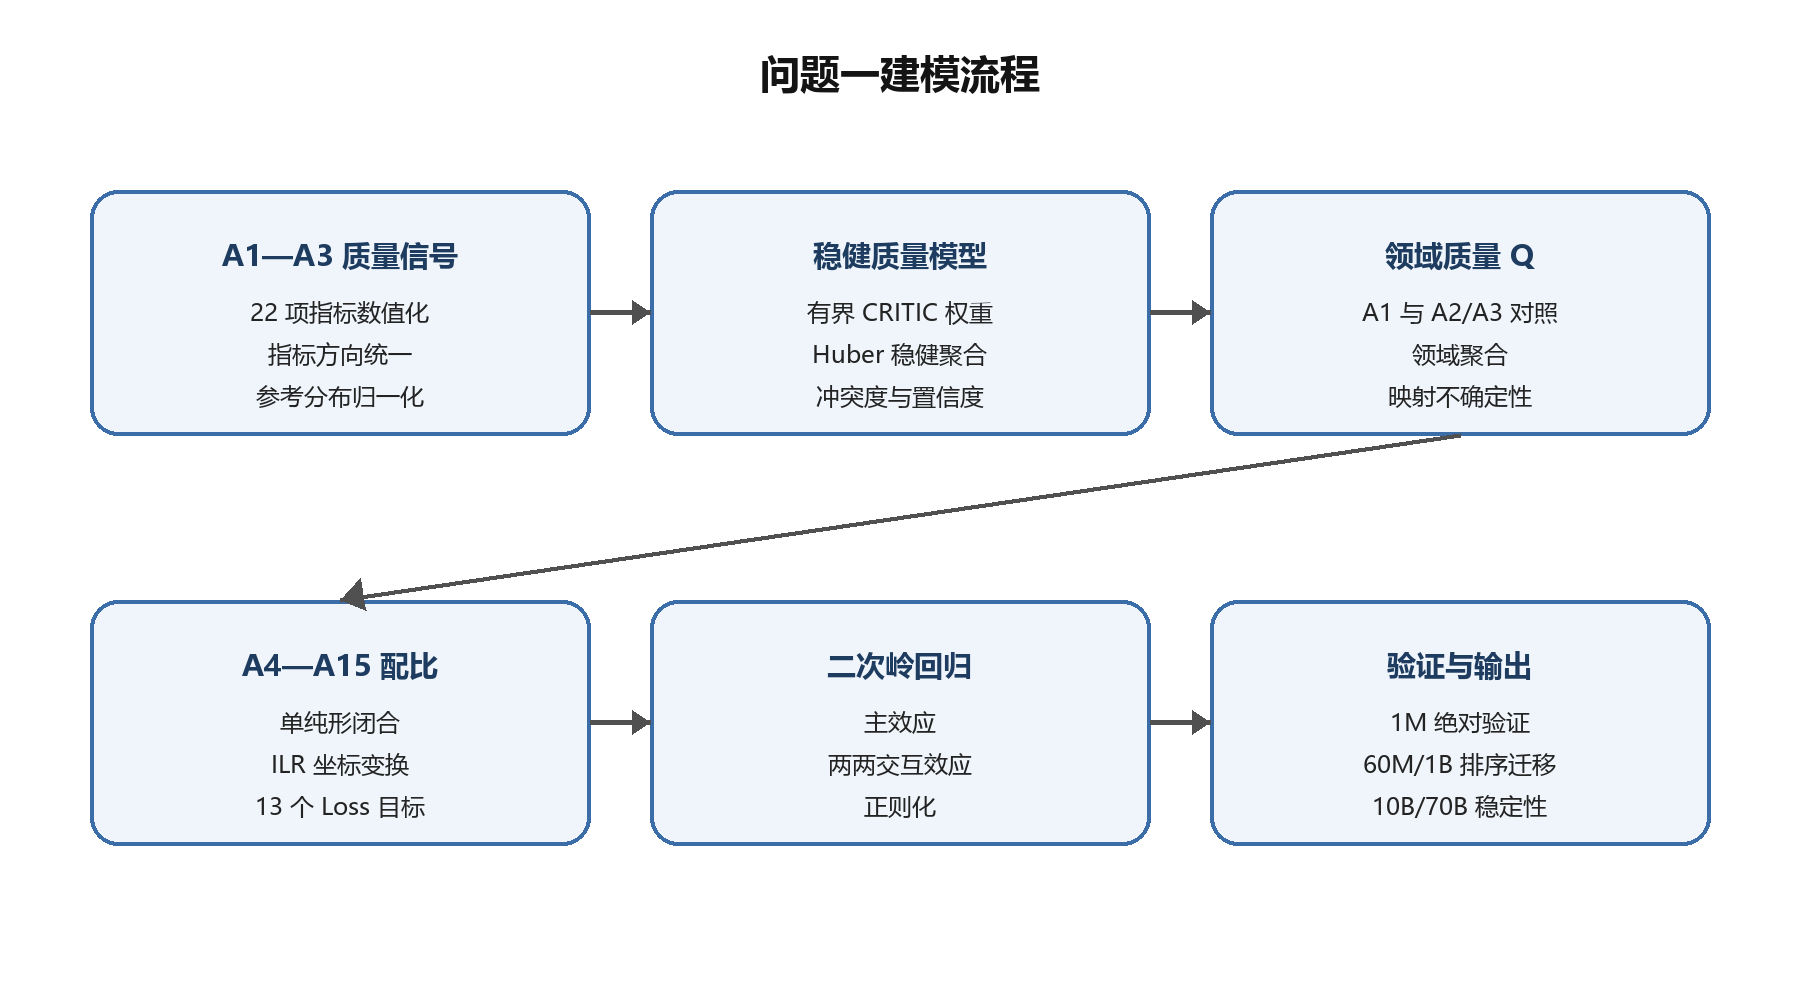
\includegraphics[width=0.96\textwidth]{figures/4.1.png}   % figure 4.1
      \caption{问题一建模流程 (待更新)}
      \label{fig:workflow}
    \end{figure}
    
    \subsection{模型建立}   % 4.2
        \subsubsection{列表型质量信号标量化}  % 4.2.1 
        设文本 $i$ 的指标 $j$ 原始输出为 $x_{ij}$。标量字段直接保留；8 个列表型字段按输出含义处理。

        对 `fluency\_en' 和 `ad\_en' 的二分类 logits $(a_0,a_1)$，取正类概率：
        \begin{equation}
        x_{ij}=\frac{\exp(a_1)}{\exp(a_0)+\exp(a_1)}.
        \label{eq:binary}
        \end{equation}
        
        对四个 `modernbert\_*' 的 6 级有序 logits，取归一化期望等级：
        \begin{equation}
        x_{ij}=\sum_{c=0}^{5}\frac{c}{5}
        \frac{\exp(a_c)}{\sum_{h=0}^{5}\exp(a_h)}.
        \label{eq:ordinal}
        \end{equation}
        
        `qurater' 的四个分量表示并列质量侧面，分别经逻辑函数后求平均：
        \begin{equation}
        x_{ij}=\frac{1}{4}\sum_{c=1}^{4}\frac{1}{1+\exp(-a_c)}.
        \label{eq:qurater}
        \end{equation}
        
        `fineweb\_edu' 的列表仅含一个元素，直接取其值。这样避免了对 logits 直接平均造成的量纲错误。


        \subsubsection{方向统一与缺失处理}   % 4.2.2 
        以 A1 为参考样本，计算指标 $j$ 的 1\%、50\%、99\% 分位数 $q_{.01,j},q_{.50,j},q_{.99,j}$，并将极端值缩尾到该区间。效益型指标转换为
        \begin{equation}
        S_{ij}=\frac{\clip(x_{ij})-q_{.01,j}}{q_{.99,j}-q_{.01,j}},
        \label{eq:benefit}
        \end{equation}
        成本型指标转换为
        \begin{equation}
        S_{ij}=1-\frac{\clip(x_{ij})-q_{.01,j}}{q_{.99,j}-q_{.01,j}}.
        \label{eq:cost}
        \end{equation}
        
        词数、句数、数字比例和平均词长设为目标型指标：
        \begin{equation}
        S_{ij}=\begin{cases}
        1-\dfrac{q_{.50,j}-x_{ij}}{q_{.50,j}-q_{.01,j}},&x_{ij}\le q_{.50,j},\\[6pt]
        1-\dfrac{x_{ij}-q_{.50,j}}{q_{.99,j}-q_{.50,j}},&x_{ij}>q_{.50,j}.
        \end{cases}
        \label{eq:target}
        \end{equation}
        所有结果截断到 $[0,1]$，从而统一为越高越好。缺失值先用同领域中位数填补，再用 A1 全局中位数兜底；另保留原始覆盖率，防止填补后的记录被误认为信息完整。
        
        
        \subsubsection{受限 CRITIC 权重}    % 4.2.3
        在方向统一后的 A1 得分上计算标准差 $\sigma_j$ 和相关系数 $\rho_{jh}$。CRITIC 方法[2]把变异性和非冗余性结合为
        \begin{equation}
        C_j=\sigma_j\sum_{h=1}^{22}(1-|\rho_{jh}|),\qquad
        w_j^{(c)}=\frac{C_j}{\sum_hC_h}.
        \label{eq:critic}
        \end{equation}
        
        为避免噪声造成权重过度集中，将 CRITIC 权重与等权重各占一半，并限制单项范围：
        \begin{equation}
        \widetilde w_j=\frac12\frac1{22}+\frac12w_j^{(c)},\qquad
        w_j=\frac{\clip(\widetilde w_j,0.5/22,2/22)}
        {\sum_h\clip(\widetilde w_h,0.5/22,2/22)}.
        \label{eq:weight}
        \end{equation}
        
        全量运行中，数字字符比例、专业性、句数、词数和流畅度权重较高，分别为 0.0609、0.0548、0.0538、0.0527 和 0.0526；全部指标仍保留正权重。

        
        \subsubsection{Huber 鲁棒综合质量分}   % 4.2.4
        若直接取加权均值，单个严重偏离的指标仍可能拉动结果。本文采用加权 Huber 位置估计[3]：
        \begin{equation}
        Q_i=\arg\min_{q\in[0,1]}\sum_{j=1}^{22}w_j
        \rho_{1.345}\!\left(\frac{S_{ij}-q}{\widehat\sigma_i}\right),
        \label{eq:huberq}
        \end{equation}
        其中
        \begin{equation}
        \widehat\sigma_i=1.4826\operatorname{median}_{j}|S_{ij}-q|,
        \qquad
        \rho_c(u)=\begin{cases}
        \tfrac12u^2,&|u|\le c,\\
        c|u|-\tfrac12c^2,&|u|>c.
        \end{cases}
        \label{eq:huber}
        \end{equation}
        通过迭代重加权求解式(4.9)。在指标一致时，该估计接近加权均值；出现少数异常指标时，其边际权重随残差增大而下降。

        
        \subsubsection{冲突定义、置信度与成因贡献}   % 4.2.5
        定义加权分歧度和稳健极差为
        \begin{equation}
        D_i=\sqrt{\sum_jw_j(S_{ij}-Q_i)^2},\qquad
        R_i=P_{90}(S_{i\cdot})-P_{10}(S_{i\cdot}).
        \label{eq:disagreement}
        \end{equation}
        
        以 A1 的 $D_i$ 的 95\% 分位数为 $\tau_D$，显著冲突定义为
        \begin{equation}
        I_i=\I(D_i>\tau_D\ \land\ R_i>0.60).
        \label{eq:conflict}
        \end{equation}
        全量计算得到 $\tau_D=0.38725$。联合条件既要求总体分歧较大，也要求指标两端存在实质距离。
        
        评分置信度定义为
        \begin{equation}
        Conf_i=Coverage_i\left(1-\min\left\{\frac{D_i}{0.50},1\right\}\right).
        \label{eq:confidence}
        \end{equation}
        
        指标 $j$ 对全部冲突的归一化贡献为
        \begin{equation}
        A_j=\frac{\E_{i:I_i=1}[w_j|S_{ij}-Q_i|]}
        {\sum_h\E_{i:I_i=1}[w_h|S_{ih}-Q_i|]}.
        \label{eq:attribution}
        \end{equation}
        该贡献只用于定位分歧来源，不把某一指标直接判定为错误。

        
        \subsubsection{领域聚合与扩展集检验}  % 4.2.6
        领域质量取领域内文本质量均值：
        \begin{equation}
        Q_d=\frac1{n_d}\sum_{i:g(i)=d}Q_i.
        \label{eq:domainq}
        \end{equation}
        同时报告均值标准误区间、冲突率和平均置信度。arxiv、github 分别比较 A1 与扩展集的均值差、Cohen's $d$ 和两样本 KS 统计量。最终领域评分中，这两个领域使用扩展集估计；其余领域使用 A1，避免 A1 与扩展集可能重合的记录被重复计数。
        
        
        \subsubsection{ILR 坐标}  % 4.2.7
        配比向量属于 16 维单纯形：
        \begin{equation}
        \bm p_i\in\mathcal S^{16}=\left\{\bm p:p_k\ge0,\ \sum_{k=1}^{17}p_k=1\right\}.
        \label{eq:simplex}
        \end{equation}
        
        对零分量加入 $\epsilon=10^{-4}$ 后重新闭合：
        \begin{equation}
        \widetilde p_{ik}=\frac{p_{ik}+\epsilon}{\sum_h(p_{ih}+\epsilon)}.
        \label{eq:closure}
        \end{equation}
        
        令 $H\in\mathbb R^{16\times17}$ 为 Helmert 正交对比矩阵，则 ILR 坐标为
        \begin{equation}
        \bm z_i=H\left(\log\widetilde{\bm p}_i-
        \frac1{17}\bm 1\bm 1^{\mathsf T}\log\widetilde{\bm p}_i\right).
        \label{eq:ilr}
        \end{equation}
        该变换保留 Aitchison 几何距离，并消除任意删去一个配比分量带来的解释依赖。

        
        \subsubsection{二次多输出岭回归}    % 4.2.8
        对 13 个验证域分别建立共享正则强度的二次响应面：
        \begin{equation}
        L_{ir}=\beta_{0r}+\bm\beta_r^{\mathsf T}\bm z_i
        +\bm z_i^{\mathsf T}\Gamma_r\bm z_i+\varepsilon_{ir}.
        \label{eq:ridge}
        \end{equation}
        参数通过
        \begin{equation}
        \min_{\beta,\Gamma}\sum_{i,r}(L_{ir}-\widehat L_{ir})^2
        +\lambda\left(\|\beta\|_2^2+\|\Gamma\|_F^2\right)
        \label{eq:ridgeobjective}
        \end{equation}
        估计。五折交叉验证在 $10^{-4}$ 至 $10^4$ 的对数网格上选择 $\lambda$，最终得到 $\lambda=10$。二次项表达领域对之间的非可加关系，岭惩罚用于控制 512 个样本下的估计方差。

        
        \subsubsection{验证指标与跨规模迁移}  % 4.2.9
        同规模检验报告 RMSE、MAE、方差加权 $R^2$ 和 13 个目标 Spearman 相关的均值。对 60M、1B，主指标为
        \begin{equation}
        \bar\rho_s=\frac1{13}\sum_{r=1}^{13}
        \operatorname{Spearman}(L_{sr},\widehat L_{1M,r}).
        \label{eq:spearman}
        \end{equation}
        
        为区分``排序可迁移''和``绝对标尺已改变''，另拟合
        $L_{sr}=a_{sr}+b_{sr}\widehat L_{1M,r}+e$ 给出描述性校准误差。该校准使用检验标签，只用于判断单调关系，不作为独立预测成绩。

        
        \subsubsection{领域边际效应与组合效应} % 4.2.10
        将领域 $k$ 的份额增加 $\delta=0.01$，其余领域按比例缩减，记为 $T_k(\bm p,\delta)$。平均边际效应为
        \begin{equation}
        ME_k=\E_{\bm p}\left[
        \frac{\bar L(T_k(\bm p,\delta))-\bar L(\bm p)}{\delta}
        \right],\qquad
        \bar L=\frac1{13}\sum_rL_r.
        \label{eq:marginal}
        \end{equation}
        
        两领域组合的二阶差分为
        \begin{equation}
        INT_{jk}=\frac{
        \bar L(T_{jk})-\bar L(T_j)-\bar L(T_k)+\bar L(\bm p)
        }{\delta^2}.
        \label{eq:interaction}
        \end{equation}
        $ME_k<0$ 表示在观测配方邻域内增加该域通常降低平均 Loss；$INT_{jk}<0$ 表示组合降低 Loss 超过可加预期。

        
        \subsubsection{质量与配比的部分识别}  % 4.2.11
        A16 只为 arxiv、github、stackexchange、wikipedia\_en、gutenberg\_pg\_19、pile\_cc 提供直接或近直接质量映射。记已映射集合为 $M$：
        \begin{equation}
        K(\bm p)=\sum_{k\in M}p_kQ_{m(k)},\qquad
        c(\bm p)=\sum_{k\in M}p_k.
        \label{eq:mapped}
        \end{equation}
        
        对未映射质量不作主观点估计，而以观测领域质量范围给出
        \begin{equation}
        Q_{mix}\in\left[K+(1-c)Q_{min},\ K+(1-c)Q_{max}\right].
        \label{eq:partial}
        \end{equation}
        中点敏感性值为
        \begin{equation}
        Q_{mix}^{mid}=K+(1-c)\bar Q.
        \label{eq:qmid}
        \end{equation}
        由于式(4.26)本身是配比的线性组合，将其与 17 个配比变量同时进入回归无法识别独立质量效应。因此本文将它用于解释覆盖度和不确定区间，不重复估计所谓``质量系数''。


    \subsection{建模结果}   % 4.3
        \subsubsection{领域质量评分} % 4.3.1
        表4.1给出最终选择的数据源和领域质量。arxiv 与 commoncrawl 的平均质量最高，均约为 0.717；github 为 0.545。book 只有 171 条记录，95\% 区间更宽且冲突率达到 56.73\%，因此其排名不宜过度解释。
    
        \begin{table}[H]    % table 4.2
        \centering
        \caption{领域质量评分与冲突率}
        \label{tab:domainq}
        \begin{tabular}{lcrrr}
        \toprule
        领域 & 最终数据源 & 样本量 & $Q$ & 冲突率/\% \\
        \midrule
        arxiv & A2 扩展集 & 17,523 & 0.71684 & 21.59 \\
        book & A1 抽样集 & 171 & 0.49113 & 56.73 \\
        c4 & A1 抽样集 & 10,000 & 0.67606 & 10.67 \\
        commoncrawl & A1 抽样集 & 9,640 & 0.71664 & 0.33 \\
        github & A3 扩展集 & 203,752 & 0.54470 & 7.15 \\
        stackexchange & A1 抽样集 & 10,000 & 0.66447 & 0.14 \\
        wikipedia & A1 抽样集 & 10,000 & 0.59758 & 3.55 \\
        \bottomrule
        \end{tabular}
        \end{table}
        
        \begin{figure}[H]
          \centering
          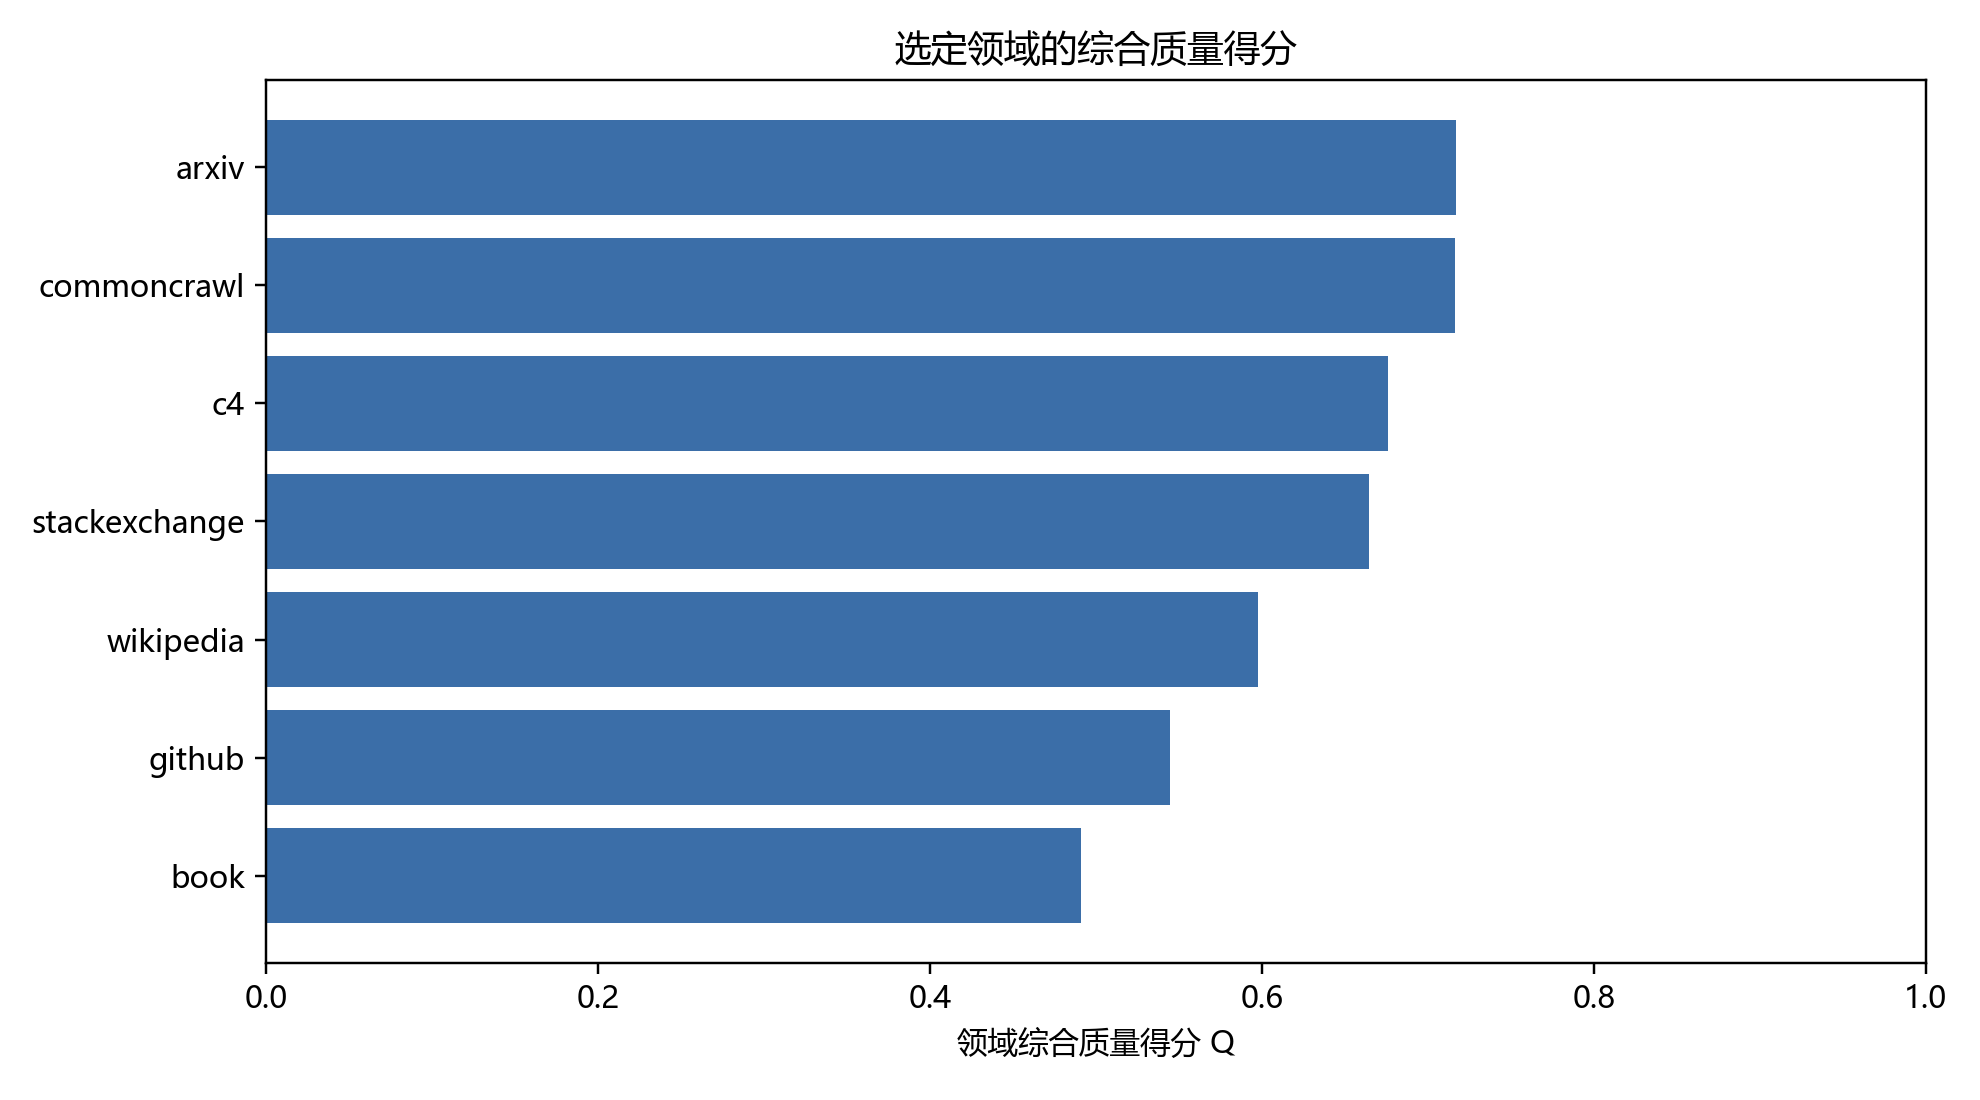
\includegraphics[width=0.92\textwidth]{figures/4.2.png}   % figure 4.2
          \caption{最终领域质量评分}
          \label{fig:qualitydomain}
        \end{figure}
        

        \subsubsection{A1 与扩展集的一致性}    % 4.3.2
        表4.3显示，arxiv 扩展集的平均质量比 A1 抽样低 0.00604，Cohen's $d=-0.0700$；github 的均值差仅 $-0.00126$，Cohen's $d=-0.0144$。arxiv 的 KS 检验因样本量大而达到统计显著，但效应量很小，不能据此声称抽样集与扩展集存在实质性质量差异。github 的分布差异也很小。扩展结果支持 A1 对这两个领域的均值代表性。
        
        \begin{table}[H]
        \centering
        \caption{A1 抽样与扩展集质量对照} % table 4.3
        \label{tab:extension}
        \begin{tabular}{lrrrrrr}
        \toprule
        领域 & $n_{A1}$ & $n_{ext}$ & $Q_{A1}$ & $Q_{ext}$ & 均值差 & Cohen's $d$ \\
        \midrule
        arxiv & 1,419 & 17,523 & 0.72287 & 0.71684 & $-0.00604$ & $-0.0700$ \\
        github & 10,000 & 203,752 & 0.54596 & 0.54470 & $-0.00126$ & $-0.0144$ \\
        \bottomrule
        \end{tabular}
        \end{table}
        
        \begin{figure}[H]
          \centering
          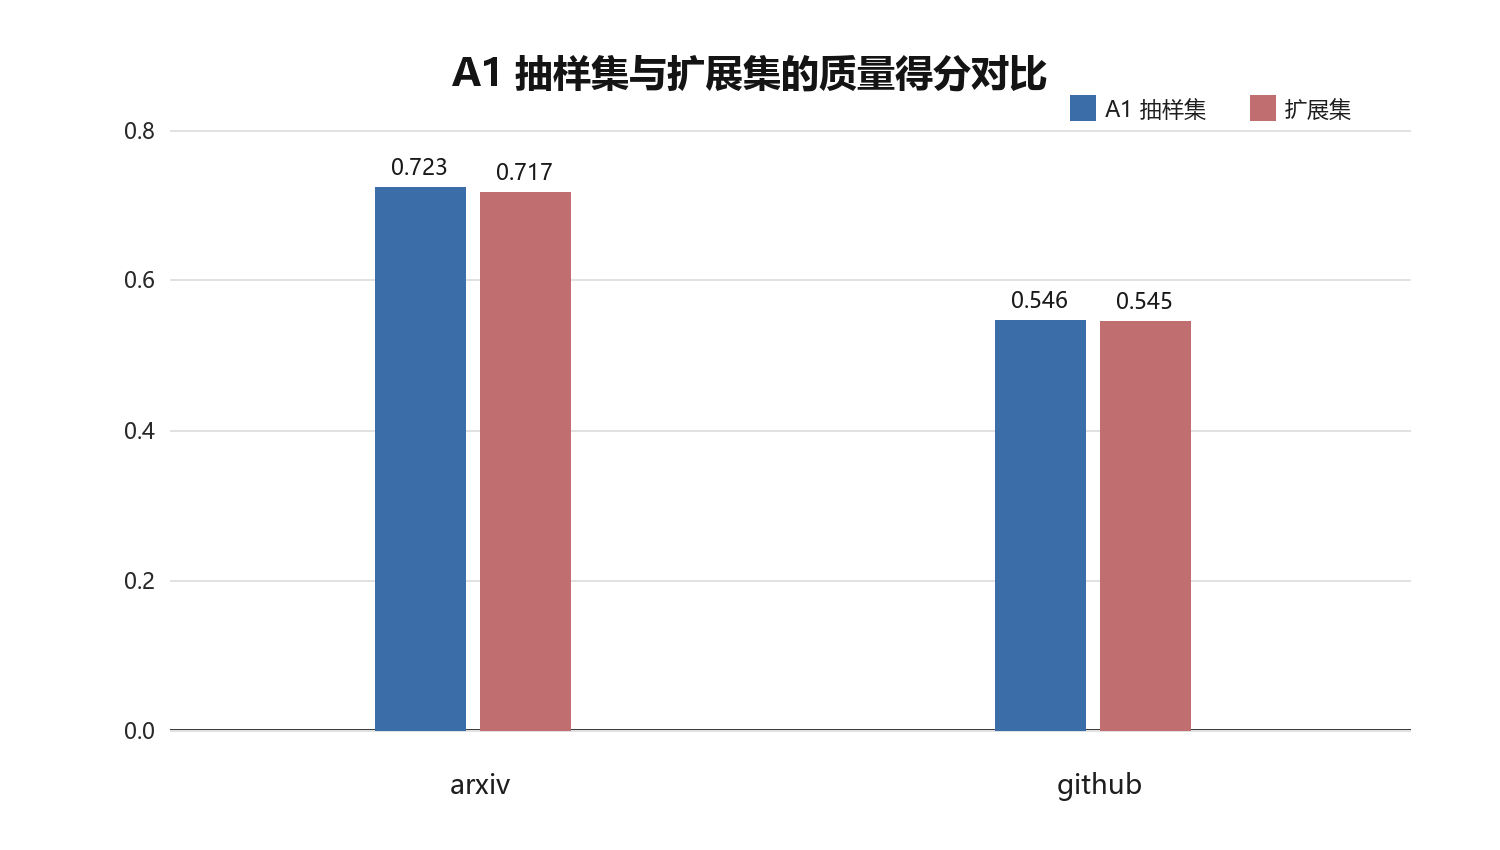
\includegraphics[width=0.80\textwidth]{figures/4.3.png}  % figure 4.3
          \caption{A1 抽样与 A2/A3 扩展集平均质量比较}
          \label{fig:extension}
        \end{figure}


        \subsubsection{冲突结构与消解结果}  % 4.3.3
        全体 272,505 条记录的冲突率为 7.675\%。冲突贡献最高的指标为数字字符比例、词数、最高频三元字符比例、句数、最高频二元字符比例和广告信号，归一化贡献分别为 0.0617、0.0607、0.0569、0.0542、0.0538 和 0.0523。该结果说明冲突主要来自文本结构、长度和重复特征与模型型质量分之间的分歧，而非某个单一指标完全失效。
        
        \begin{figure}[H]
          \centering
          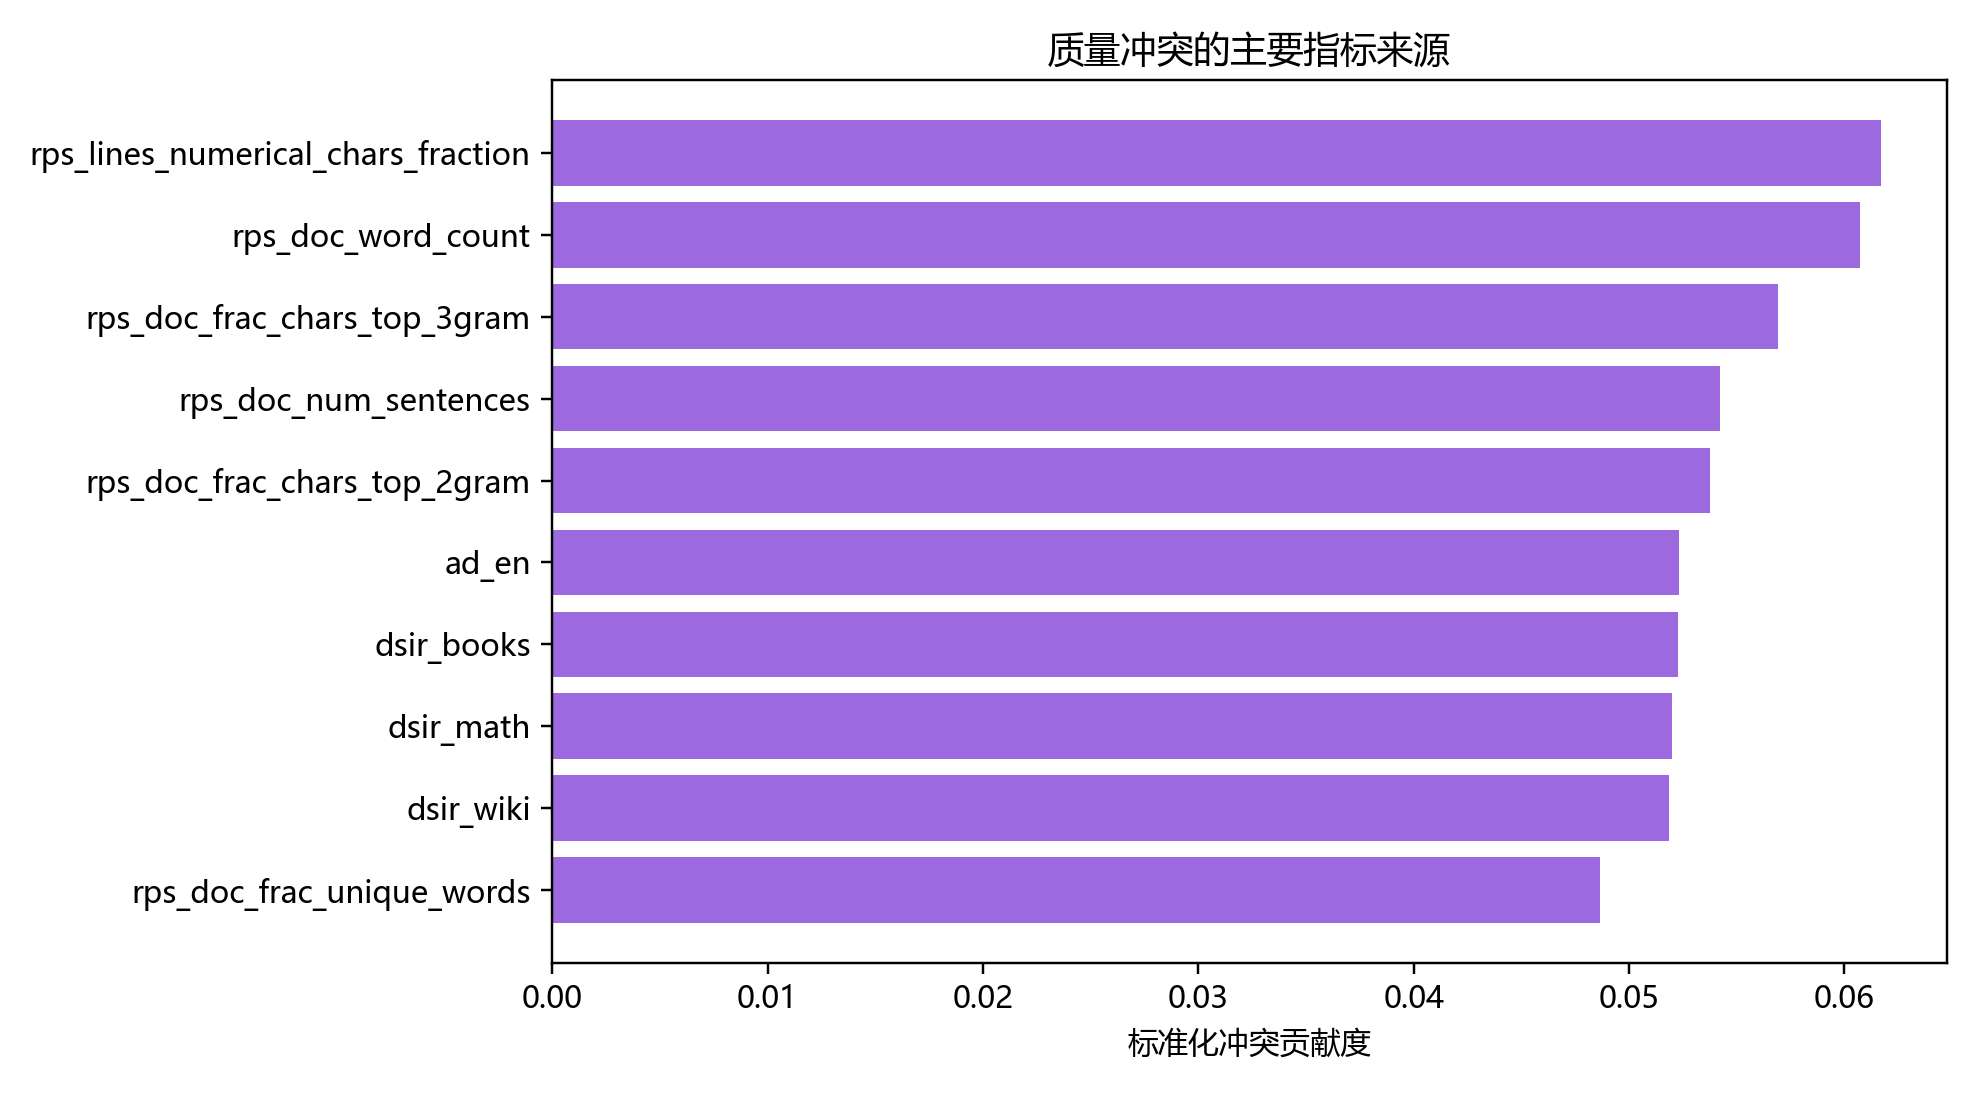
\includegraphics[width=0.93\textwidth]{figures/4.4.png}   % figure 4.4
          \caption{冲突记录中的主要指标贡献}
          \label{fig:conflictcontrib}
        \end{figure}
        
        Huber 聚合在冲突样本中降低大残差指标的有效权重，同时保留文本记录和其余指标。相比``检测冲突后删除样本''，该处理不会系统性排除包含公式、代码或特殊格式的高价值文本。置信度 $Conf_i$ 则将分歧程度和原始覆盖率显式保留下来，便于后续模型使用质量分时进行筛选或加权。


        \subsubsection{配比模型验证} % 4.3.4
        表8.5给出三组真实检验结果。1M 同规模检验取得 RMSE 0.28465、MAE 0.20269、$R^2=0.86473$，平均 Spearman 为 0.93396，说明二次 ILR 岭回归能够同时解释多数验证域的配比差异。
        
        60M 和 1B 的未校准 $R^2$ 为负，原因是模型规模改变了绝对 Loss 基准，而非配方排序失效。二者的平均 Spearman 仍为 0.92950 和 0.84253。使用检验标签做每个目标的一维仿射校准后，$R^2$ 分别达到 0.85178 和 0.81292；该结果只说明单调结构可通过尺度和平移校准，不视为独立预测性能。
        
        \begin{table}[H]
        \centering
        \caption{A6--A11 配比模型验证结果}  % table 4.4
        \label{tab:validation}
        \begin{threeparttable}
        \begin{tabular}{lrrrrrr}
        \toprule
        检验集 & RMSE & MAE & $R^2$ & 平均 Spearman & 校准 RMSE & 校准 $R^2$ \\
        \midrule
        1M & 0.28465 & 0.20269 & 0.86473 & 0.93396 & 0.27409 & 0.87458 \\
        60M & 1.59999 & 1.50659 & $-7.30804$ & 0.92950 & 0.21371 & 0.85178 \\
        1B & 2.70008 & 2.62433 & $-189.99642$ & 0.84253 & 0.08450 & 0.81292 \\
        \bottomrule
        \end{tabular}
        \begin{tablenotes}\small
        \item 注：60M、1B 的仿射校准使用相应检验标签，只用于描述跨规模单调迁移，不是独立预测。
        \end{tablenotes}
        \end{threeparttable}
        \end{table}
        
        \begin{figure}[H]   % figure 4.5
          \centering
          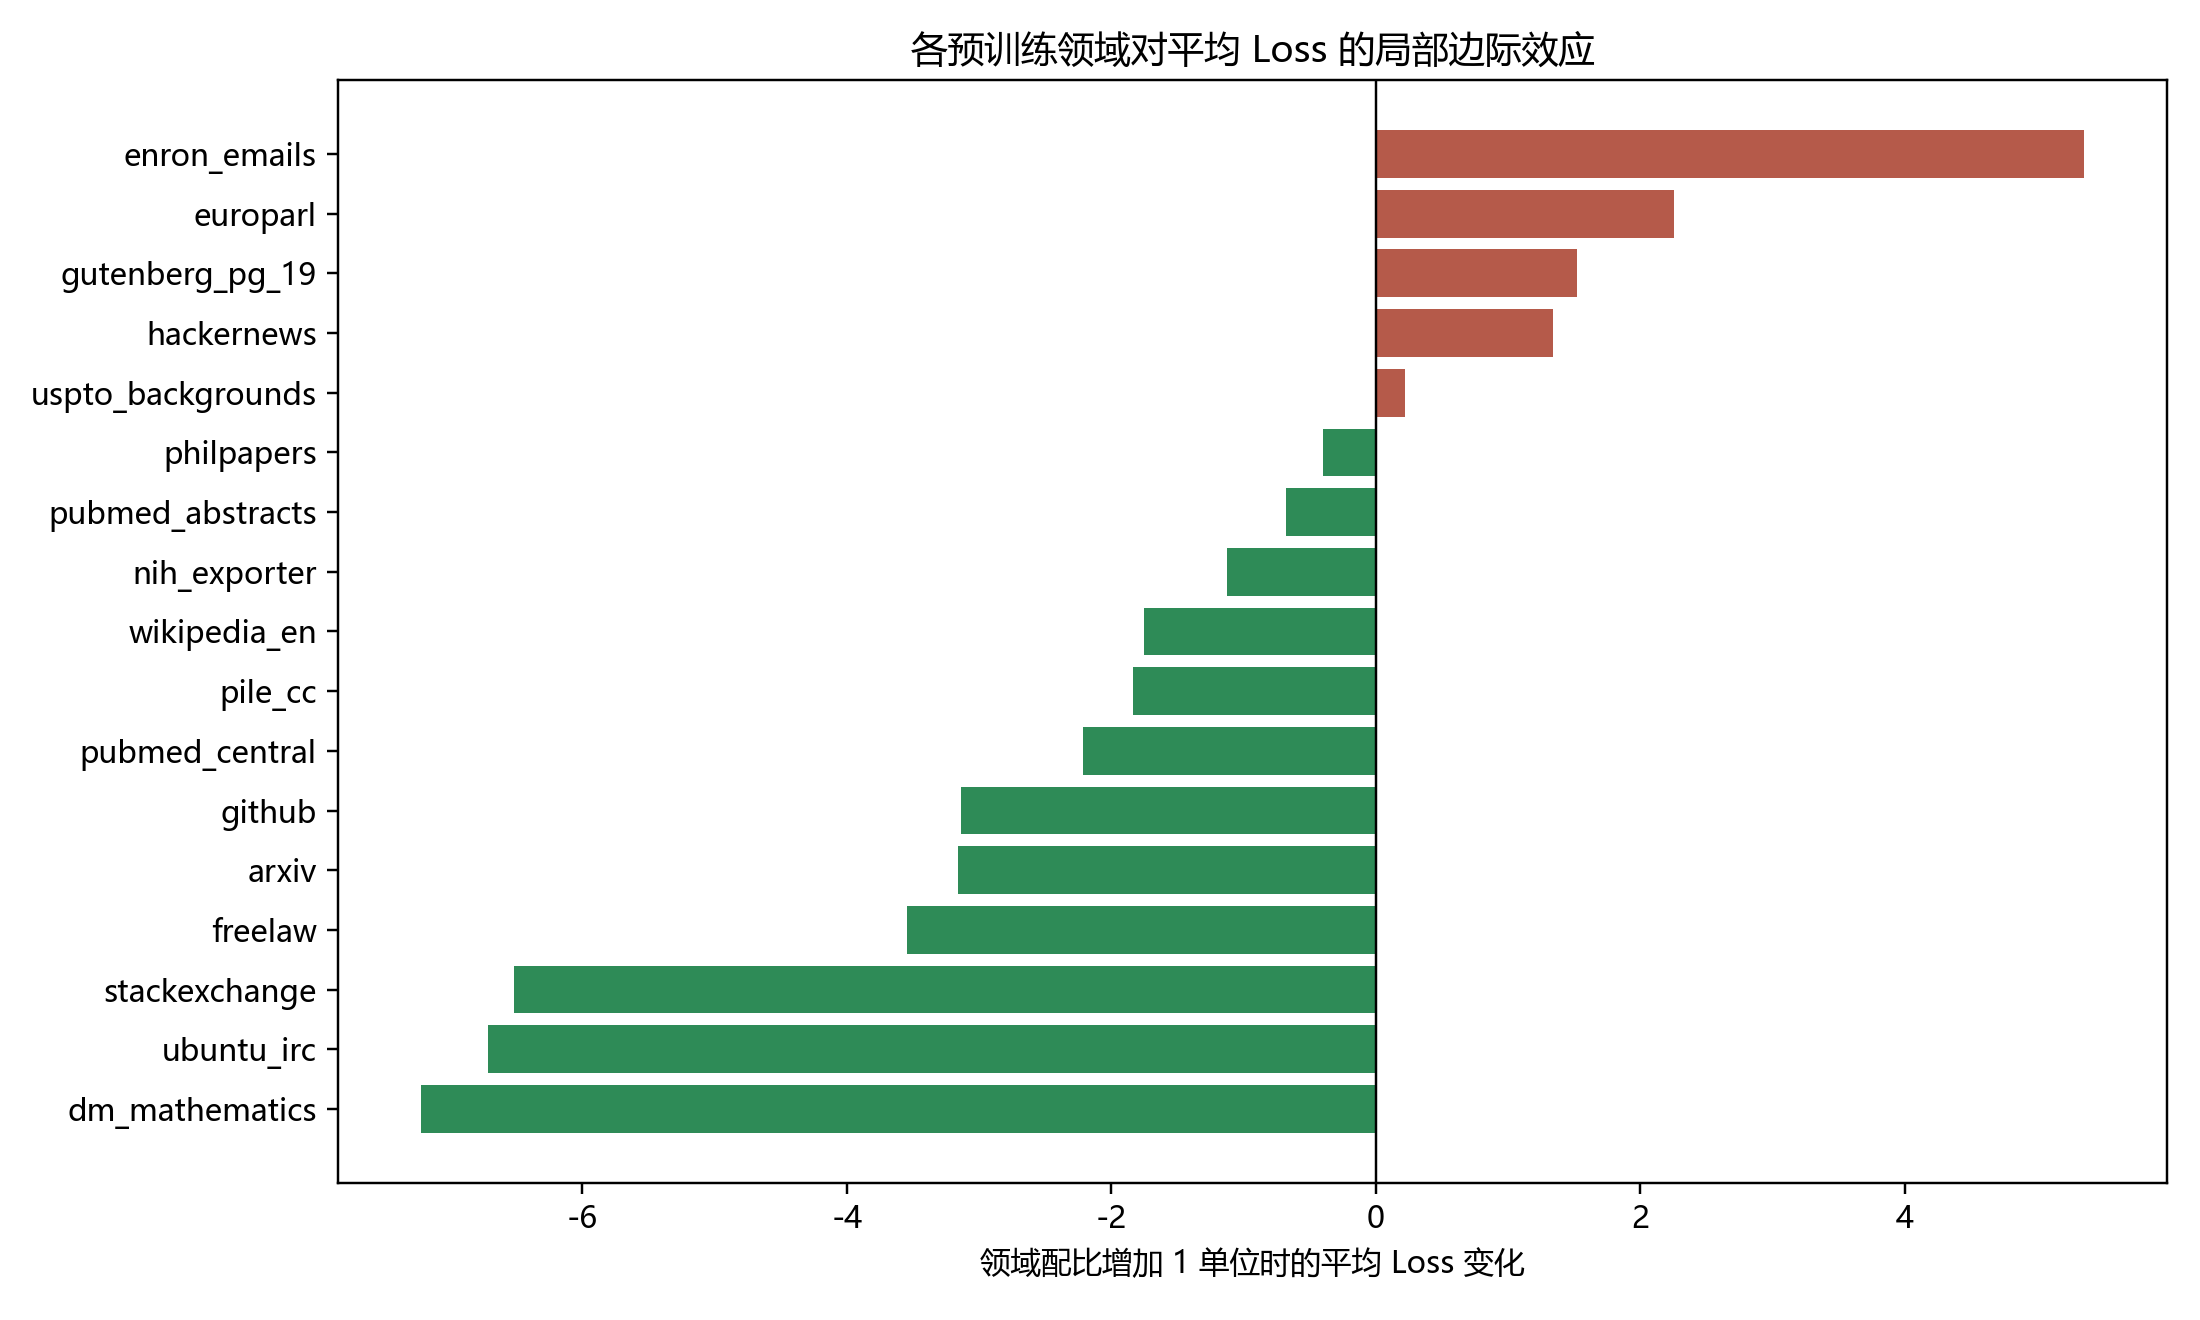
\includegraphics[width=0.78\textwidth]{figures/4.5.png}  % figure 4.5
          \caption{不同参数规模下的配方排序迁移}
          \label{fig:spearman}
        \end{figure}


        \subsubsection{领域主效应} % 4.3.5
        图4.5展示在 200 个训练配方附近计算的平均局部导数。dm\_mathematics、ubuntu\_irc、stackexchange 的平均导数分别为 $-7.216$、$-6.711$、$-6.515$，即增加 1 个百分点份额时，平均 Loss 的预测变化约为 $-0.0722$、$-0.0671$、$-0.0651$。enron\_emails、europarl 和 gutenberg\_pg\_19 的导数为正。由于不同参考配方下的导数标准差较大，这些数值应理解为样本分布上的平均局部关联。
        
        \begin{table}[H]
        \centering
        \caption{绝对值较大的领域局部边际效应}    % table 4.5    
        \label{tab:effects}
        \begin{tabular}{lrrl}
        \toprule
        领域 & $ME_k$ & 标准差 & 局部解释 \\
        \midrule
        dm\_mathematics & $-7.216$ & 7.897 & 增加份额通常降低 Loss \\
        ubuntu\_irc & $-6.711$ & 7.256 & 增加份额通常降低 Loss \\
        stackexchange & $-6.515$ & 9.119 & 增加份额通常降低 Loss \\
        enron\_emails & 5.354 & 14.464 & 增加份额通常提高 Loss \\
        freelaw & $-3.545$ & 8.092 & 增加份额通常降低 Loss \\
        arxiv & $-3.160$ & 6.573 & 增加份额通常降低 Loss \\
        github & $-3.139$ & 7.928 & 增加份额通常降低 Loss \\
        europarl & 2.252 & 8.100 & 增加份额通常提高 Loss \\
        \bottomrule
        \end{tabular}
        \end{table}
        
        \begin{figure}[H]
          \centering
          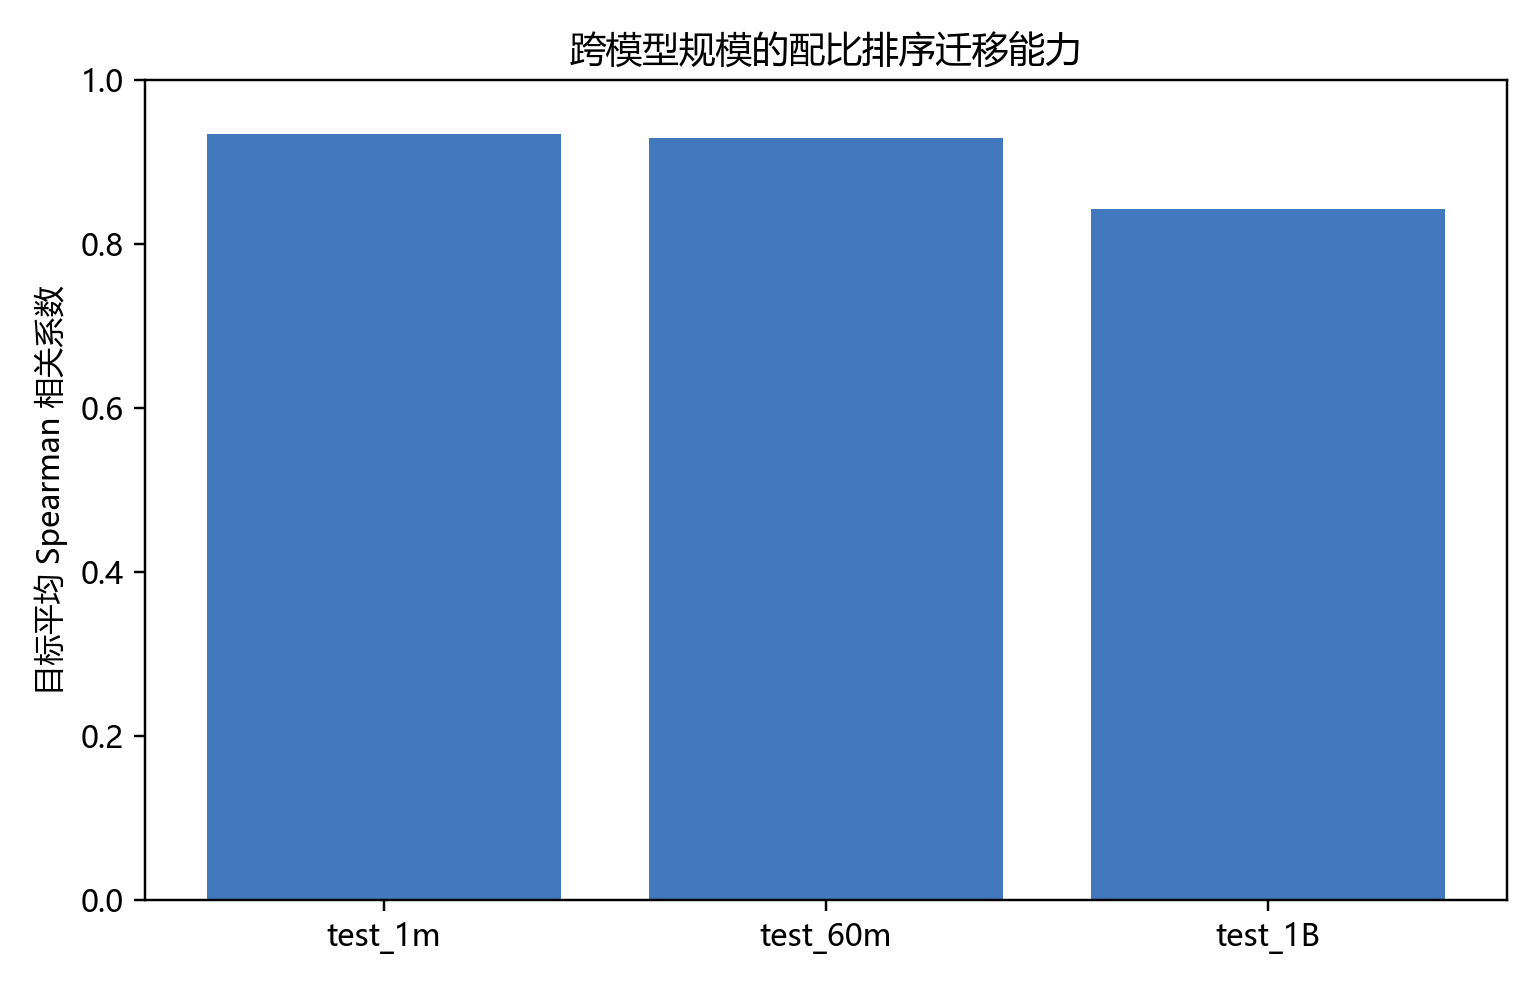
\includegraphics[width=0.96\textwidth]{figures/4.6.png}   % figure 4.6
          \caption{17 个训练领域对平均 Loss 的局部边际效应}
          \label{fig:maineffect}
        \end{figure}


        \subsubsection{领域组合效应} % 4.3.6
        二阶差分绝对值最大的组合多涉及样本中较稀疏的 philpapers、nih\_exporter 和 enron\_emails。例如 philpapers--enron\_emails 的 $INT=87.85$，表示组合效果弱于主效应可加预期；enron\_emails--europarl 的 $INT=-18.33$，表现为局部协同。由于二阶效应对配方位置和伪计数更敏感，本文只把其作为筛选需要进一步实验的领域组合，不把数值直接解释为稳定因果效应。
        
        \begin{table}[H]
        \centering
        \caption{绝对值最大的领域组合效应}  % table 4.6
        \label{tab:interactions}
        \begin{tabular}{llrr}
        \toprule
        领域 1 & 领域 2 & $INT_{jk}$ & 类型 \\
        \midrule
        philpapers & enron\_emails & 87.85 & 拮抗 \\
        nih\_exporter & philpapers & 59.38 & 拮抗 \\
        nih\_exporter & enron\_emails & 51.52 & 拮抗 \\
        enron\_emails & hackernews & 44.71 & 拮抗 \\
        philpapers & europarl & 27.07 & 拮抗 \\
        enron\_emails & europarl & $-18.33$ & 协同 \\
        enron\_emails & gutenberg\_pg\_19 & 17.38 & 拮抗 \\
        nih\_exporter & europarl & 13.44 & 拮抗 \\
        \bottomrule
        \end{tabular}
        \end{table}


        \subsubsection{质量映射覆盖与不可辨识性}    % 4.3 7
        A16 的直接或近直接映射只覆盖 6 个配方域。训练配方的平均已映射质量为 0.5646，1M/60M 检验为 0.5690，1B 为 0.6224；不同配方的覆盖质量从接近 0 到 1 不等。训练集的 $Q_{mix}$ 部分识别区间平均宽度为 0.0983，1M/60M 为 0.0973，1B 为 0.0852。该宽度表明，对未映射 11 域强行填入单一质量分会制造不可忽略的模型确定性。本文因此保留上下界，并将 $Q_{mix}^{mid}$ 只作为敏感性描述量。
        
        \begin{table}[H]
        \centering
        \caption{配方质量映射覆盖情况}    % table 4.7
        \label{tab:mapping}
        \begin{tabular}{lrrrr}
        \toprule
        数据集 & 样本量 & 平均映射质量 & 最小--最大映射质量 & 平均区间宽度 \\
        \midrule
        训练 1M & 512 & 0.5646 & 0.000--1.000 & 0.0983 \\
        检验 1M & 256 & 0.5690 & 0.001--1.000 & 0.0973 \\
        检验 60M & 256 & 0.5690 & 0.001--1.000 & 0.0973 \\
        检验 1B & 64 & 0.6224 & 0.138--0.888 & 0.0852 \\
        外推 10B/70B & 各 63 & 0.5435 & 0.003--1.000 & 0.1030 \\
        \bottomrule
        \end{tabular}
        \end{table}


        \subsubsection{外推稳定性}   % 4.3.8
        A12--A15 上的未校准绝对误差很大，符合模型规模改变 Loss 基准的预期。10B 和 70B 的配方排序平均 Spearman 分别为 0.60949 和 0.52874；使用外推标签做仿射校准后 $R^2$ 分别为 0.57882 和 0.45793。该结果说明效应排序具有中等稳定性，但明显弱于真实 60M/1B 检验。由于外推配比为训练子集、Loss 也来自外推，本文不把它作为真实大模型实验验证。
        
        \begin{table}[H]
        \centering
        \caption{A12--A15 外推稳定性结果}  % table 4.8
        \label{tab:extrapolation}
        \begin{tabular}{lrrrr}
        \toprule
        数据集 & 未校准 RMSE & 平均 Spearman & 校准 RMSE & 校准 $R^2$ \\
        \midrule
        10B 外推 & 3.62349 & 0.60949 & 0.17124 & 0.57882 \\
        70B 外推 & 4.01115 & 0.52874 & 0.16192 & 0.45793 \\
        \bottomrule
        \end{tabular}
        \end{table}


        \subsubsection{小结}  % 4.3.9
        本节完成了问题一的质量评价、冲突消解和领域配比建模。基于 272,505 条记录构建的 Huber 综合质量分能够统一 22 个异质指标。arxiv 与 commoncrawl 的领域质量最高，github 与 book 较低；book 的样本量和冲突结构使其不确定性更大。总体冲突率为 7.675\%。冲突主要与数字比例、文本长度和重复统计有关。Huber 估计能够在不删除文本的情况下抑制离群指标。arxiv、github 的扩展集与 A1 抽样集平均质量差异很小，Cohen's $d$ 的绝对值均小于 0.08，支持 A1 的均值代表性ILR 二次岭回归在 1M 检验集上达到 $R^2=0.86473$，跨到 60M 和 1B 后配方排序相关仍为 0.92950 和 0.84253。配比规律主要以相对排序形式迁移，绝对 Loss 需要规模校准在观测配方邻域内，dm\_mathematics、ubuntu\_irc、stackexchange 的平均边际效应最有利；enron\_emails 的平均效应不利。该结论仅适用于局部调整。A16 的映射覆盖不足以识别独立质量系数。部分识别区间比主观补值更诚实，也为问题二引入质量因素提供了不确定性边界。


\section{问题二}   % 5
    \subsection{问题分析}

    \subsection{模型建立}

    \subsection{建模结果}

\section{问题三}   % 6
    \subsection{问题分析}

    \subsection{模型建立}

    \subsection{建模结果}

\section{问题四}   % 7
    \subsection{问题分析}

    \subsection{模型建立}

    \subsection{建模结果}

\section{模型评价}  % 8 (1~3 pages)
模型评价


\begin{thebibliography}{9}  % 参考文献
 \bibitem{bib:one} ...参考一
 \bibitem{bib:two} ...参考二
\end{thebibliography}


\clearpage


\begin{appendices}  % 附录
    % \setcounter{page}{1}  % 如果需要可以自行重置页码。
    \section{MATLAB 源程序}    % 附录 A
    \renewcommand{\thesubsection}{A\thinskip.\thinskip\arabic{subsection}}
        \subsection{第1问程序}  % A.1
        \vspace{-2ex}
        
        \begin{Matlab}{code.m}
        clear all
        kk=2;
        [mdd,ndd]=size(dd);
        while ~isempty(V)
            [tmpd,j]=min(W(i,V));
            tmpj=V(j);
            for k=2:ndd
                [tmp1,jj]=min(dd(1,k)+W(dd(2,k),V));
                tmp2=V(jj);
                tt(k-1,:)=[tmp1,tmp2,jj];
            end
            tmp=[tmpd,tmpj,j;tt];
            [tmp3,tmp4]=min(tmp(:,1));
            if tmp3==tmpd,
                ss(1:2,kk)=[i;tmp(tmp4,2)];
            else
                tmp5=find(ss(:,tmp4)~=0);
                tmp6=length(tmp5);
                if dd(2,tmp4)==ss(tmp6,tmp4)
                    ss(1:tmp6+1,kk)=[ss(tmp5,tmp4);tmp(tmp4,2)];
                else, ss(1:3,kk)=[i;dd(2,tmp4);tmp(tmp4,2)];
                end
            end
            dd=[dd,[tmp3;tmp(tmp4,2)]];
            V(tmp(tmp4,3))=[];
            [mdd,ndd]=size(dd);kk=kk+1;
        end;
        S=ss; D=dd(1,:);
        \end{Matlab}
        \vspace{2ex}
    
    \clearpage
    \section{Python 源程序}    % 附录 B
    \renewcommand{\thesubsection}{B\thinskip.\thinskip\arabic{subsection}}
        \subsection{第2问程序}  % B.1
        \vspace{-2ex}
        \begin{Python}{mip1.py}
        # This example formulates and solves the following  MIP model:
        #  maximize
        #        x +   y + 2 z
        #  subject to
        #        x + 2 y + 3 z <= 4
        #        x +   y       >= 1
        #        x, y, z binary
        
        # import gurobipy as gp
        from gurobipy import * #GRB
        try:
            # Create a new model
            m = Model("mip1")
            # Create variables
            x = m.addVar(vtype=GRB.BINARY, name="x")
            y = m.addVar(vtype=GRB.BINARY, name="y")
            z = m.addVar(vtype=GRB.BINARY, name="z")
            # Set objective
            m.setObjective(x + y + 2 * z, GRB.MAXIMIZE)
            # Add constraint: x + 2 y + 3 z <= 4
            m.addConstr(x + 2 * y + 3 * z <= 4, "c0")
            # Add constraint: x + y >= 1
            m.addConstr(x + y >= 1, "c1")
            # Optimize model
            m.optimize()
            for v in m.getVars():
                print('%s %g' % (v.varName, v.x))
            print('Obj: %g' % m.objVal)
        
        except GurobiError as e:
            print('Error code ' + str(e.errno) + ': ' + str(e))
        
        except AttributeError:
            print('Encountered an attribute error')
        \end{Python}
    
\end{appendices}


\end{document} 